\setAuthor{Jaan Kalda}
\setRound{piirkonnavoor}
\setYear{2015}
\setNumber{G 9}
\setDifficulty{8}
\setTopic{Magnetism}

\prob{Magnetväli}
Piirkonnas $0<y<a$ on $z$-teljega paralleelne homogeenne magnetväli induktsiooniga $B$; piirkondades $y<0$ ja $y>a$ magnetväli puudub. 
Osake massiga $m$ ja laenguga $q$ siseneb kiirusega $v$ magnetväljaga piirkonda paralleelselt $y$-teljega üle joone $y=0$. Visandage osakese kiirusvektori ja $y$-telje vaheline nurk pärast seda, kui osake on piirkonnast $0<y<a$ väljunud funktsioonina kiirusest $v$.

\hint
Laeng sooritab magnetväljas ringliikumist; mida suurem on magnetväli, seda suurem on ringi raadius. Enne ja pärast ringliikumist on osakese trajektoor sirge, kusjuures ülemine ringjooneks on ilma murdepunktita, st sirgjooned on ringjoone puutujaks.

\solu
\begin{center}
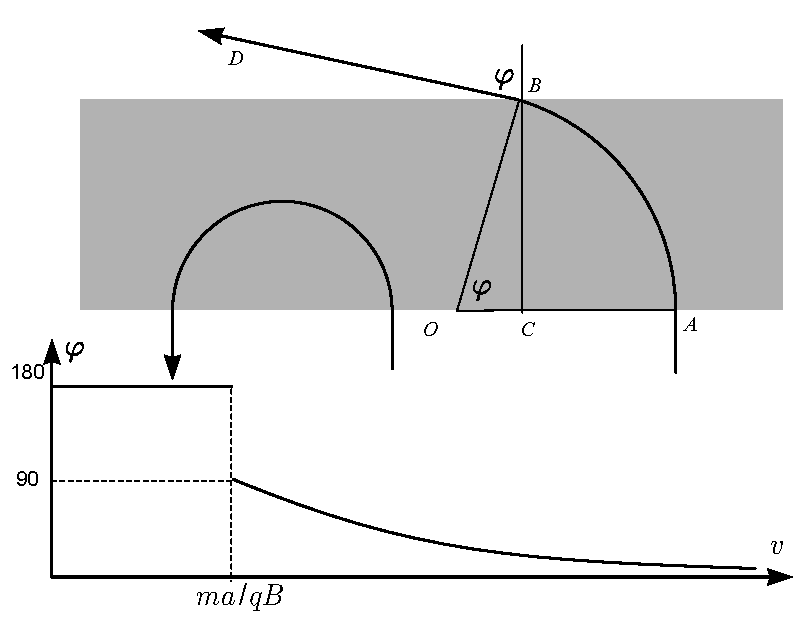
\includegraphics[width=0.7\textwidth]{2015-v2g-09-magnetvalilah}
\end{center}
Laeng sooritab magnetväljas ringliikumist, vt joonis;
ringi raadiuse leiame Newtoni II seadusest $Bqv=mv^2/R$, millest
$R=\frac{mv}{qB}$. Enne ja pärast ringliikumist on trajektooriks sirge, kusjuures üleminek ringjooneks on ilma murdepunktita, st sirgjooned on ringile puutujaks. Väikeste kiiruste korral, kui $R<a$, st $v<\frac{Bqa}{m}$, siis läheb osake otse tagasi,
st väljumisnurk $\varphi=\pi \SI{}{rad}=180^\circ$.

Väljudes on kiirusvektor risti ringi raadiusega, st $\angle OBD=\frac \pi 2$, mistõttu $\varphi=\angle COB$. Seega,
\[
\varphi=\arcsin \frac{BC}{BO}=\arcsin \frac{a}{R}=\arcsin \frac{qBa}{mv}.
\]

\probeng{Magnetic field}
In the region $0<y<a$ there is a $z$-directional homogenous magnetic field with an induction $B$, in the regions $y<0$ and $y>a$ there is no magnetic field. A particle with a mass $m$ and a charge $q$ enters the magnetic field with a speed $v$ parallel to the $y$-axis over the line $y=0$. Sketch the angle between the particle’s velocity and the $y$-axis after when the particle has exited the region $0<y<a$ as a function of the speed $v$.

\hinteng
The charge performs a circular motion in the magnetic field; the bigger the magnetic field the bigger the radius of the circle. Before and after the circular motion the trajectory of the particle is linear, moreover the linear lines are the tangents of the circle.

\solueng
\begin{center}
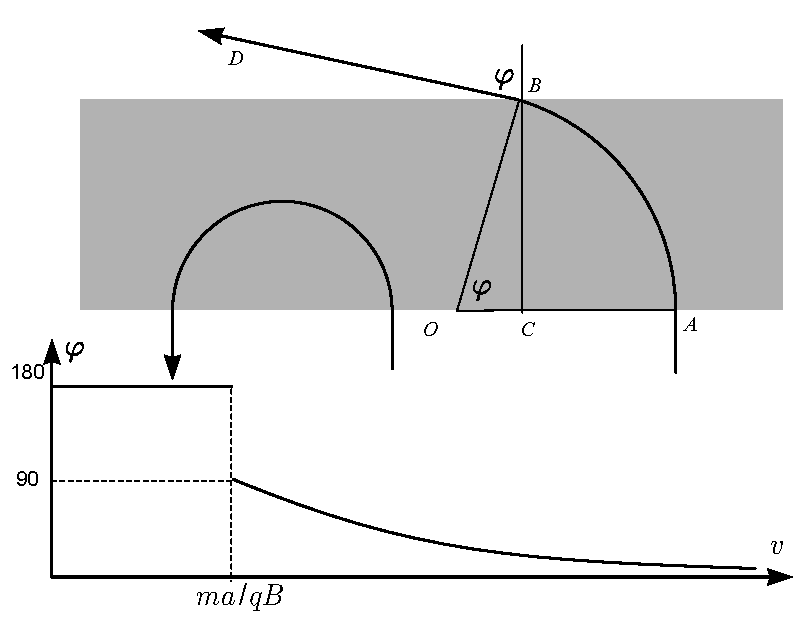
\includegraphics[width=0.7\textwidth]{2015-v2g-09-magnetvalilah}
\end{center}
The particle performs a circular movement in the magnetic field, see figure; we find the radius of the ring from the Newton’s second law $Bqv=mv^2/R$ where $R=\frac{mv}{qB}$. Before and after the circular movement the trajectory is a line, moreover the transition into a circle is without a breakpoint, meaning that the lines are the circle’s tangent. For small velocities, if $R<a$, meaning $v<\frac{Bqa}{m}$, then the particle goes straight back, meaning that the exiting angle is $\varphi=\pi \SI{}{rad}=180^\circ$.\\
When exiting the magnetic field the velocity’s vector is perpendicular to the circle’s radius, meaning $\angle OBD=\frac \pi 2$, which is why $\varphi=\angle COB$. Therefore $\varphi=\arcsin \frac{BC}{BO}=\arcsin \frac{a}{R}=\arcsin \frac{qBa}{mv}$.
\probend